Nesse capítulo, serão apresentados as Equações que regem os fenômenos geomecânicos. O primeiro trabalho famoso na modelagem de tensões no solo é Terzaghi que desenvolveu a teoria para uma dimensão. Mais tarde, Biot generalizou essa teoria para três dimensões e essas são as Equações que serão apresentadas. Detalhes das duas teorias podem ser encontradas em \citet{CompGeomec}. Como intuito do trabalho é testar o método multiescala aplicado para matrizes dessa natureza, o caso aqui considerado será o de elasticidade linear onde a rocha não é tensionada até que apresente falhas. O capítulo \ref{ch:discretizacao} apresentará como as equações aqui encontradas são resolvidas utilizando o método dos elementos finitos.



\section{Tensor de Tensões}

Para representar a tensão total (ou \textit{overburden}) em um ponto da rocha, é utilizado um tensor de tensões de segunda ordem como mostra \eqref{eq:tensordetensoes}.

\begin{equation} \label{eq:tensordetensoes}
\mathbf{\sigma} =
    \begin{bmatrix}
    \stxx & \stxy & \stxz \\
    \styx & \styy & \styz \\
    \stzx & \stzy & \stzz
    \end{bmatrix}
\end{equation}

O primeiro subscrito do tensor representa a face que a tensão está sendo aplicada, enquanto o segundo representa a direção da tensão. A figura \ref{fig:tensoesx} mostra as componentes com o com primeiro subscrito x.


\begin{figure}[!htbp]
\centering
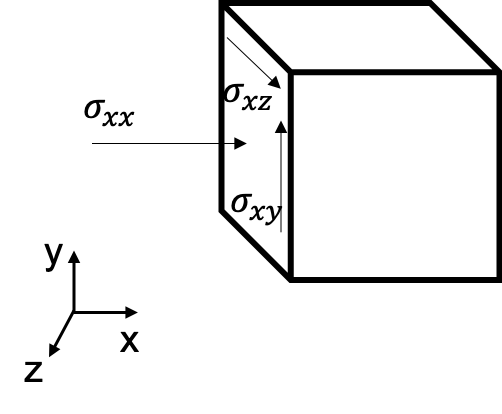
\includegraphics[width=5cm]{chap01/figs/tensor.png}
\caption{Tensões $\sigma_{x.}$ representadas graficamente.}
\label{fig:tensoesx}
\end{figure}

Ao aplicar a condição de equilíbrio do momento angular, chega-se a conclusão que $\stxy=\styx$, $\stxz=\stzx$ e $\styz=\stzy$. Dessa maneira, para a representação desse tensor, são necessários guardar apenas seis valores. Pode-se considerar então a tensão como o vetor apresentado \label{eq:tensor6} essa notação é chamada de notação de Voigt e é a bastante utilizada nas implementações de elementos finitos, por exemplo, nas formulações apresentadas por \cite{hughes} e \cite{jacob}.


\begin{equation}
\sigma^T = \begin{bmatrix}
\stxx & \styy & \stzz & \stxy & \stxz & \styz
\end{bmatrix}
\label{eq:tensor6}
\end{equation}


\section{Teoria da Consolidação}

Para um certo elemento de volume $\Delta x\Delta y \Delta z$ pode-se escrever as equações de equilíbrio para cada uma dessas direções. A Figura \ref{fig:equilibrio} apresenta todas as tensões relativas a direção x.

\begin{figure}[!htbp]
\centering
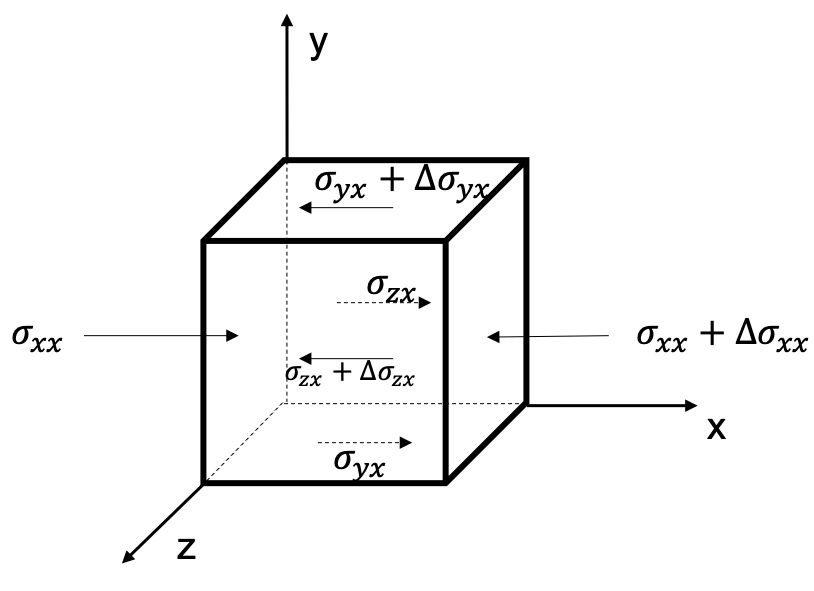
\includegraphics[width=8cm]{chap01/figs/equilibrio.png}
\caption{Tensões na direção x ($\sigma_{.x}$) representadas graficamente.  Adaptado de \cite{CompGeomec}.}
\label{fig:equilibrio}
\end{figure}

O equilíbrio de forças nessa direção pode ser escrito como apresentado em \eqref{eq:equilibrio0}. Nesse caso as forças atuantes são calculadas a partir da tensão multiplicada pela área de atuação. Sobre o valor $f_x$, ele, juntamente com os termos $f_y$ e $f_z$  são termos gravitacionais e representam a força peso do volume $\Dx\Dy\Dz$. Como apresentado em ??? (colocar referência de doutorado) $\mathbf{f} = [\rho_s(1-\phi) + \phi(\rho_o S_o + \rho_w S_w + \rho_g S_g )] \mathbf{g}$ onde $\phi$ é a porosidade, $S_o$, $S_w$ e $S_g$ as saturações de óleo, água e gás e $\rho_o$, $\rho_w$, $\rho_g$  as densidades do óleo, água e gás. Esse termo será considerado constante ao longo da simulação realizada nesse trabalho, fazendo com que as modificações no equilíbrio serão apenas relativas a mudança de pressão.


\begin{multline} \label{eq:equilibrio0}
   (\stxx - \stxx - \Delta \stxx) \Dy\Dz + (\styx - \styx - \Delta \styx)\Dx\Dz  +\\
   + (\stzx - \stzx - \Delta\stzx) \Dx\Dy + f_x\Dx\Dy\Dz = 0
\end{multline}


\begin{equation}
 \Delta \stxx \Dy\Dz + \Delta \styx\Dx\Dz + \Delta\stzx - f_x\Dx\Dy\Dz = 0
\end{equation}

Dividindo todos os termos por $\Dx\Dy\Dz$.


\begin{equation}
\frac{ \Delta \stxx }{ \Dx } + \frac{\Delta \styx}{ \Dy } + \frac{\Delta\stzx}{ \Dz } - f_x = 0
\end{equation}

Fazendo $\Dx \rightarrow 0$, $\Dy \rightarrow 0 $ e $\Dz \rightarrow 0$

\begin{equation}
\dx[\stxx] + \dy[\styx] + \dy[\stzx] - f_x = 0
\end{equation}

Analogamente, para as direções y e z pode-se encontrar a equação de equilíbrio também, montando o sistema \eqref{eq:equilibrio1}.

\begin{equation}
\label{eq:equilibrio1}
\left\{\begin{matrix}
 \dx[\stxx] + \dy[\styx] + \dz[\stzx] - f_x & = & 0\\
 \dx[\stxy] + \dy[\styy] + \dz[\stzy] - f_y & = & 0\\
 \dx[\stxz] + \dy[\styz] + \dz[\stzz] - f_z & = & 0
\end{matrix}\right.
\end{equation}


As tensões apresentadas em \eqref{eq:equilibrio1} são as tensões totais que atuam no cubo infinitesimal. Acontece que ao tratar de reservatórios de petróleo, estes possuem fluído no volume poroso da rocha (óleo, água e gás) como mostra a Figura \ref{fig:rochaComFluido} e, portanto, parte da tensão total será suporta pelo fluído e parte será suportado pelos grãos da rocha. Como fluído não oferece resistência ao cisalhamento, ele suporta apenas parte das tensões $\stxx$, $\styy$ e $\stzz$.

\begin{figure}[!htbp]
\centering
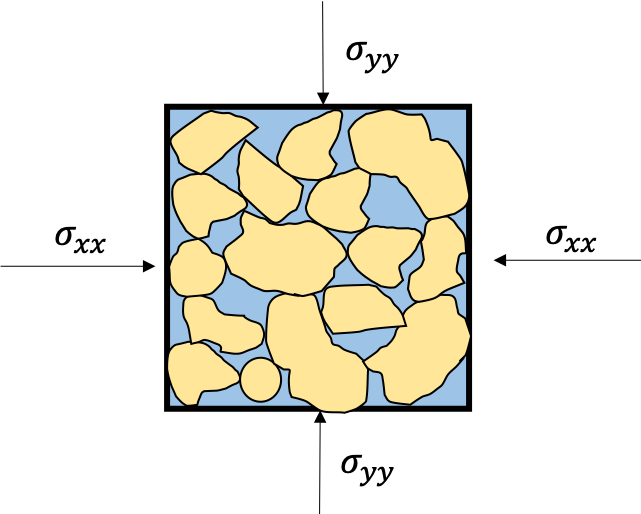
\includegraphics[width=7cm]{chap01/figs/fluido_rocha_tensoes.png}
\caption{Figura de meio poroso, grãos amarelos representando a matriz da rocha e fluído representado por cor azul}
\label{fig:rochaComFluido}
\end{figure}

Para isso pode-se utilizar a teoria de consolidação de poroelasticidade desenvolvida por Biot,  \citet{}, para três dimensões que mostra que a tensão efetiva na rocha ($\sigma^{\prime\prime}$) e a tensão total são relacionadas por \eqref{eq:tensaoefetiva} conforme mostrado em \citet{ResGeomec}.

\begin{equation}
\label{eq:tensaoefetiva}
    \sigma^{\prime\prime} = \sigma - \alpha P_p
\end{equation}

Onde $\sigma^{\prime\prime}$ é a tensão efetiva, $\alpha$ é o coeficiente de Biot e $P_p$ a pressão de poros. O coeficiente de Biot representa o quanto a pressão de poros do fluído suporta a tensão total na rocha e está no intervalo $\alpha \in [0,1]$.

Assim, as equações \eqref{eq:equilibrio1} podem ser reescritas como \eqref{eq:equilibrio} substituindo as tensões totais ($\sigma$) pela tensões efetivas na rocha ($\sigma^\prime$). Essas equações são encontras em \cite{CompGeomec}.



\begin{equation}
\label{eq:equilibrio}
\left\{\begin{matrix}
\dx[\sxx]  + \dy[\syx] + \dz[\szx] - \dx[\alpha P_p] + f_x   = 0
\\
\dx[\sxy]  + \dy[\syy] + \dz[\szy] - \dy[\alpha P_p]  + f_y   = 0
\\
\dx[\sxz]  + \dy[\syz] + \dz[\szz] - \dz[\alpha P_p] + f_z   = 0
\end{matrix}\right.
\end{equation}

Ou ainda, escrevendo utilizando os operadores divergente, gradiente e $f^T=\begin{bmatrix}f_x & f_y & f_z\end{bmatrix}$ a Equação pode ser rescrita como \eqref{eq:equilibrio_matriz}.
\begin{equation}
\label{eq:equilibrio_matriz}
\nabla \cdot \stef - \nabla \alpha P_p + f = 0
\end{equation}

Por motivos de implementação mais eficiente menor uso de memória e utilização de operações mais simples (multiplicação de matrizes por vetores) a Equação \eqref{eq:equilibrio_matriz} pode ser escrita na notação de Voigt  considerando as definições conforme \eqref{eq:equilibrio_final}.

\begin{equation}
\label{eq:equilibrio_final}
\sopnabla^T \stef - \sopnabla^T\alpha m  P_p - f = 0
\end{equation}

Onde,
\begin{equation}
\begin{matrix}\label{eq:definicoesvoigt}
\stef = \begin{bmatrix}
\sxx
\\
\syy
\\
\szz
\\
\sxy
\\
\sxz
\\
\syz
\end{bmatrix}
&

;

&

f = \begin{bmatrix}
f_{x}
\\
f_{y}
\\
f_{z}
\end{bmatrix}
&
;
&

m = \begin{bmatrix} 1 \\ 1 \\ 1 \\ 0 \\ 0 \\ 0\end{bmatrix}

&
;

&
\sopnabla = \sop
\end{matrix}
\end{equation}



\subsection{Relações Constitutivas}

A Equação \eqref{eq:equilibrio_final} apresenta o equilíbrio em função das tensões, porém, pelo grande número de variáveis dessa equação é necessário colocar em função das variáveis de deslocamento. O Campo de deslocamentos será representado pela variável $\deslocamento = [u_x \quad u_y \quad u_z]^T$. A deformação ($\deformacao$) se relaciona com o deslocamento de acordo com \eqref{eq:defor_desloc}. A relação entre a deformação e as tensões é definida como relação constitutiva de acordo com \citet{ResGeomec}.

\begin{equation}
\label{eq:defor_desloc}
\deformacao = \sopnabla \deslocamento
\end{equation}


Vários tipos de relações constitutivas podem ser utilizadas para representar essa relação entre tensão e deformação. A Figura \ref{fig:stress_strain} mostram dados de um teste típico de tensão-deformação em uma rocha bem cimentada. Nesse caso, é importante notar que existe um comportamento linear dominante na parte central do gráfico antes da falha. Essa região onde as deformações e tensões se relacionam linearmente é chamada de elástica, que será a região de estudo desse trabalho. %TODO talvez citar um pouco das regições de faha


\begin{figure}[!htbp]
\centering
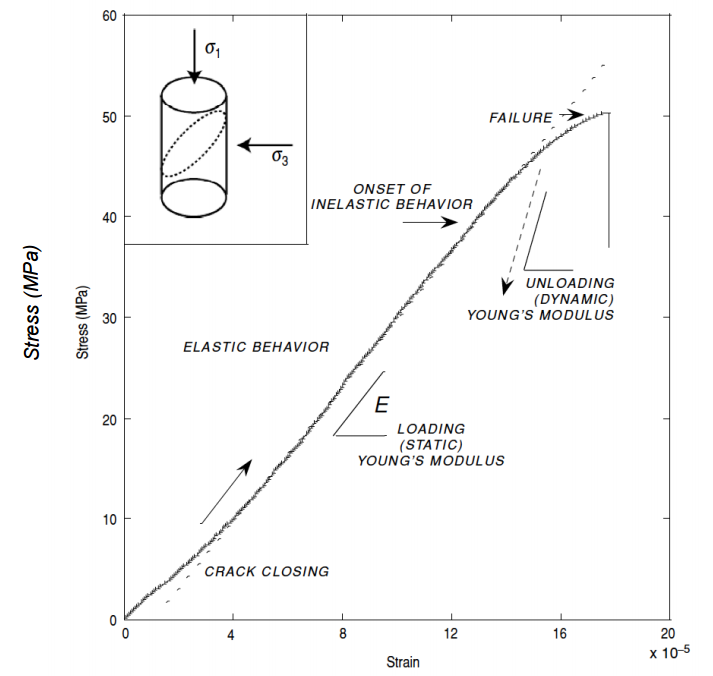
\includegraphics[width=7cm]{chap01/stress_strain.PNG}
\caption{Teste de laboratório tensão-deformação para uma rocha bem cimentada. Adaptada de \cite{ResGeomec}.}
\label{fig:stress_strain}
\end{figure}


O estudo de mecânica dos sólidos nos mostra que, na região elástica e materiais isotrópicos, é possível escrever uma relação entre as deformações e tensões nos elementos de forma simples. Essa relação é denominada de Lei de Hooke Generalizada e é apresentada na Equação \eqref{eq:hooke}. E a Equação \eqref{eq:elasticMatrix} apresenta a matriz de elasticidade.


\begin{equation}{
\label{eq:hooke}
\fontsize{4}{4}\selectfont
\sigma ^{\prime\prime}= D \epsilon
}
\end{equation}




Onde $E$ é o módulo de Young da rocha e $v$ o módulo de de Poisson. Já as deformações se relacionam com os deslocamentos pela equação \eqref{eq:defor_desloc}.

\begin{equation}
\label{eq:defor_desloc}
\epsilon = \sopnabla u
\end{equation}


A EDP da equação \eqref{eq:equilibrio_final} pode então ser escrita em função dos deslocamentos substituindo as equações \eqref{eq:hooke} e \eqref{eq:defor_desloc}.

\begin{equation}
\label{eq:edp_geomec}
\sopnabla^TD \sopnabla u - \sopnabla^T\alpha m P_p - f = 0
\end{equation}

Onde $D$ é a matriz de elasticidade da Lei de Hooke. Essa forma será a utilizada junto dos métodos do elementos finitos para construção de um simulador para regime permanente de geomecânica em duas dimensões. Ao se passar
de três dimensões para duas dimensões existem duas abordagens possíveis de stress plano ou deformação plana. Que são apresentadas respectivamente em \eqref{eq:elasticplanestress} e \eqref{eq:elasticplanestrain}.

\begin{equation} \label{eq:elasticplanestress}
D_{stress} = \frac{E}{1-\upsilon^2}
\begin{bmatrix}
1  & \upsilon & 0 \\
\upsilon & 1 &  0 \\
0 & 0 & \frac{1-\upsilon}{2}
\end{bmatrix}
\end{equation}

\begin{equation} \label{eq:elasticplanestrain}
D_{strain} = \frac{E}{(1+\upsilon)(1-2\upsilon)}
\begin{bmatrix}
 1-\upsilon & \upsilon    &  0 \\
 \upsilon   &  1-\upsilon &  0 \\
 0& 0 & \frac{1-2\upsilon}{2}
\end{bmatrix}
\end{equation}

De acordo com \cite{jacob}, a condição de deformação plana é melhor aplicada quando o elemento é grosso em relação ao plano xy que é o caso dos reservatórios de petróleo.  Dessa forma, artigos como \cite{planeStrainProblems}, \cite{casteletto} e \cite{irina} utilizam a hipótese de deformação plana que será a mesma utilizada nesse trabalho.

Os operadores e vetores devem então ser redefinidos para os mostrados em \eqref{eq:vetores2d}.

\begin{equation}
\label{eq:vetores2d}
\begin{matrix}
\sigma^\prime = \begin{bmatrix}
\sxx
\\
\syy
\\
\sxy
\end{bmatrix}
&

;

&

f = \begin{bmatrix}
f_{x}
\\
f_{y}
\end{bmatrix}
&
;
&

m = \begin{bmatrix} 1 \\ 1 \\ 0\end{bmatrix}

&
;

&
\sopnabla = \soptwod

&
;

&

u = \begin{bmatrix}
u_x
\\
u_y
\end{bmatrix}

\end{matrix}
\end{equation}

Além da Equação \eqref{eq:edp_geomec}, são necessárias as condições de contorno para que o problema fique totalmente definido.
